\documentclass[conference]{IEEEtran}

\usepackage[utf8]{inputenc}
\usepackage[T1]{fontenc}
\usepackage{graphicx,url}
\usepackage{booktabs}
\usepackage{amsmath}
\usepackage{array}
\usepackage{cite}
\usepackage{subcaption}
\usepackage{tikz}
\expandafter\def\expandafter\UrlBreaks\expandafter{\UrlBreaks\do\-\do\_}
\usetikzlibrary{shapes.geometric, arrows.meta, positioning, calc, fit, backgrounds}

% --- Vertical-space compaction (to fit the page limit) ---
\usepackage[indentafter]{titlesec}
\titlespacing*{\section}{0pt}{1.0ex plus .2ex minus .2ex}{0.6ex plus .1ex}
\titlespacing*{\subsection}{0pt}{0.7ex plus .2ex minus .2ex}{0.3ex plus .1ex}
\titlespacing*{\subsubsection}{0pt}{0.4ex plus .1ex minus .1ex}{0pt}
\renewcommand{\arraystretch}{0.9}
\setlength{\abovedisplayskip}{3pt}
\setlength{\belowdisplayskip}{3pt}
\setlength{\abovedisplayshortskip}{0pt}
\setlength{\belowdisplayshortskip}{0pt}
\setlength{\skip\footins}{5pt plus 2pt minus 1pt}
\AtBeginDocument{%
  \let\oldthebibliography\thebibliography
  \renewcommand{\thebibliography}[1]{\oldthebibliography{#1}%
    \setlength{\itemsep}{0pt}\setlength{\parsep}{0pt}\setlength{\parskip}{0pt}}}
\setlength{\textfloatsep}{4pt plus 2pt minus 2pt}
\setlength{\floatsep}{4pt plus 2pt minus 2pt}
\setlength{\intextsep}{4pt plus 2pt minus 2pt}
\setlength{\dblfloatsep}{4pt plus 2pt minus 2pt}
\setlength{\dbltextfloatsep}{4pt plus 2pt minus 2pt}
\setlength{\abovecaptionskip}{2pt}
\setlength{\belowcaptionskip}{0pt}

\sloppy

\begin{document}

\title{A Hierarchical Attack Detection Solution for 6G MEC-based IoT Networks}



\author{\IEEEauthorblockN{ Luiz Henrique B. A. da Silva\IEEEauthorrefmark{1}, José R. de Souza Silva\IEEEauthorrefmark{1},
Caio B. B. de Souza\IEEEauthorrefmark{1}\IEEEauthorrefmark{2},
and Andson M. Balieiro\IEEEauthorrefmark{1}}

\IEEEauthorblockA{\textit{\IEEEauthorrefmark{1}Centro de Informática (CIn), Universidade Federal de Pernambuco (UFPE), Recife, Brazil.    } \\
\IEEEauthorrefmark{2} Universidade de Pernambuco (UPE), Brazil.    }

\{lhbas, jrss, cbbs, amb4\}@cin.ufpe.br, caiobruno.souza@upe.br}

\maketitle

\begin{abstract}
The growth of Internet of Things (IoT) devices and the emergence of
sixth-generation (6G) networks introduce new cybersecurity challenges in
Multi-access Edge Computing (MEC) environments. This work proposes and
implements a two-phase hierarchical Intrusion Detection System (IDS) for
IoT/MEC environments: Phase~1 runs a binary LightGBM classifier on the edge
node, optimized by the $F_2$-score, and Phase~2 classifies the attack type
with a multiclass LightGBM, both fed by a pipeline that converts PCAP captures
from two CIC datasets into a 190~GB SQLite database with \textit{netflower}, a
flow extractor developed for this project. To keep detection from stalling
packet capture under flooding, inference is decoupled from capture: a separate
worker consumes flows from an unbounded queue and runs both phases in batches.
In a fully scripted testbed validation on a VIM~4 edge node covering all eight
attack categories, detection is scored \emph{per flow}, labelling each flow by
the attack window in which it started, which makes the metric independent of the
flow-extractor emission delay (median 181--428~s). Over a calibrated ($+2$~s)
window the binary IDS reaches a precision of 97\% at a recall of 70\% (F1 81\%),
strongest on volumetric floods (spoofing 95\%, DoS 90\%) and weaker on DDoS
(56\%) and low-volume attacks, whose single-packet flows fall below the 0.9
threshold. Phase~2 separates reconnaissance (F1 75\%) but merges the remaining
categories onto DoS (macro-F1 19\%). Most consequentially, the measurements
expose a throughput ceiling: at $\sim$1{,}050 flows/s the VIM~4 cannot process
traffic in real time and buffers it, with a mean end-to-end latency of 116~s for
the binary pipeline and 343~s for the hierarchical one, adding Phase~2 roughly
tripling this latency while raising average power from 3.4 to 5.1~W.
\end{abstract}

\begin{IEEEkeywords}
6G, MEC, IoT, intrusion detection, LightGBM, edge computing.
\end{IEEEkeywords}

%─────────────────────────────────────────────────────────────────────────────
\section{Introduction}

The convergence of sixth-generation (6G) mobile networks, the Internet of Things (IoT) and Multi-access Edge Computing (MEC) promises to transform the digital communication infrastructure, with estimated densities of $10^6$ IoT devices per km² and latencies below 1~ms, where MEC acts as an essential technology to meet these requirements~\cite{you:21}.

The massive proliferation of IoT devices expands the cyberattack surface and introduces severe security challenges, as these endpoints with limited resources cannot support traditional, computationally demanding security solutions. Consequently, Intrusion Detection Systems (IDSs) relying on rules and signatures have been shifted to edge nodes to bring threat detection closer to the network periphery, ensuring high detection accuracy for known threats~\cite{lazarevic:05}. Nevertheless, novel attacks and zero day variants can easily evade signature detection mechanisms, requiring frequent manual updates and human intervention, which makes this paradigm fundamentally incompatible with the 6G scale.

Machine learning (ML)-based IDSs deployed at the network edge have emerged as a promising alternative, capable of classifying network flows in real time and generalizing to unseen attack patterns with low inference overhead~\cite{gyamfi:22}. For instance, classifiers trained on Canadian Institute for Cybersecurity (CIC) IoT datasets have achieved high detection accuracy in \cite{houichi:25,chen:24}. Furthermore, recent works propose collaborative edge-cloud architectures~\cite{yang:23} and two-stage frameworks that filter traffic using a lightweight classifier before activating more computationally intensive models~\cite{aldaej:24}. Despite these advances, critical challenges remain. Most existing studies rely on datasets collected in controlled environments, risking severe distribution shifts when deployed under real network conditions. Many solutions are evaluated in cloud environments, thereby overlooking the strict energy and computational constraints of actual embedded devices. Additionally, the attack heterogeneity, coupled with conflicting optimization objectives, strongly motivates the adoption of hierarchical approaches.

To address these challenges, this work proposes a two-phase hierarchical intrusion detection system (IDS) for IoT/MEC environments. Phase 1 utilizes a lightweight binary classifier to isolate malicious traffic, which then triggers a Phase 2 multiclass classifier to categorize the specific attack type. The primary contributions of this paper include the design of this hierarchical, ML-based architecture, alongside a reproducible, SQLite-based data pipeline optimized for large-scale balanced sampling. Furthermore, this work introduces \textit{NetFlower}, a parallel tool for converting PCAP traces into network flows, which has been made publicly available on PyPI. The final core contribution consists of an experimental validation on a Khadas VIM4 embedded platform under real online traffic, comprehensively evaluating CPU, RAM, energy, and throughput, which characterizes the throughput ceiling of the hierarchical pipeline on an ARM edge node under volumetric attack and empirically identifies the point where the 55 adopted flow features lose their discriminatory effectiveness.


%Intrusion Detection Systems (IDS) based on rules and signatures have been deployed on edge nodes to bring detection closer to IoT devices, achieving high precision on known threats~\cite{lazarevic:05}, but novel attacks or variants match no recorded signature and cross the detector without raising an alert, and keeping the rule set up to date requires constant manual intervention, impractical at the scale foreseen for 6G. Machine-learning IDS running at the edge emerge as an alternative: trained on historical data, they classify flows in real time and generalize to unseen patterns at low inference cost~\cite{gyamfi:22}. Classifiers trained on IoT datasets from the Canadian Institute for Cybersecurity (CIC) achieve high detection accuracy~\cite{houichi:25,chen:24}, collaborative architectures distribute detection between edge and cloud~\cite{yang:23}, and two-stage schemes filter traffic with a lightweight classifier before triggering a more expensive one~\cite{aldaej:24}. Still, data captured in controlled environments induce distribution shift with respect to real traffic, and the diversity of attacks demands distinct optimization objectives per layer, which motivates a hierarchical approach.


%Keeping the detector on the edge node itself, rather than in the cloud, is attractive precisely on the 6G horizon: it avoids backhauling traffic for inspection, keeps the reaction latency within the access network and preserves the locality that MEC introduces~\cite{you:21}. The counterpart is that an access-tier node offers a few ARM cores, a limited amount of RAM and a power envelope of a few watts, shared between detection and the services the node hosts; a viable IDS must therefore be judged not only by its detection metrics, but also by the CPU, memory and energy it subtracts from the node~\cite{chinnasamy:25}. This coupling between accuracy and cost is what a hierarchical organization exploits: a cheap first stage inspects all the traffic, and a more informative second stage runs only on what the first one flags.


The remainder of the paper covers related work (Section~\ref{relatedWork}), the
methodology (Section~\ref{sec:methodology}), the results
(Section~\ref{sec:results}) and the conclusion (Section~\ref{sec:conclusion}).

%─────────────────────────────────────────────────────────────────────────────
\section{Related Work}
\label{relatedWork}

IDS can be signature-based, which identify known patterns with high precision
but cannot detect new threats, or anomaly-based, which learn a profile of
normal behavior and flag deviations~\cite{lazarevic:05}. Combining both
approaches in hierarchical architectures is a interesting alternative for
resource-constrained environments such as IoT devices and MEC
nodes~\cite{zolanvari:19}. Regarding anomaly-based solutions, CIC datasets have been widely used to train and evaluate IDS in IoT networks. For instance, by adpting the CIC IoT Dataset 2023~\cite{neto:23}, which reproduces a
topology of 105 devices with 33 attacks in seven categories, Houichi et~al.~\cite{houichi:25} compare classical classifiers for smart-city security, and Chen et~al.~\cite{chen:24} combine LightGBM with feature selection by an improved salp swarm algorithm. These works, however, report
only offline metrics on the dataset's own test split, without evaluating the
model deployed on a real edge node or the shift between dataset and production
traffic. Gyamfi and Jurcut~\cite{gyamfi:22} review IDS design combining MEC,
machine learning and datasets, and Yang et~al.~\cite{yang:23} propose
detection through cloud--edge collaboration. In such architectures, however,
the heaviest stage is typically moved to the cloud, and the cost of keeping
detection on the edge node itself, in CPU, RAM and energy, is rarely measured.
Aldaej et~al.~\cite{aldaej:24} propose a two-stage IDS for IoT-edge platforms. Our proposal shares this philosophy, but both phases run on the same edge node and the marginal cost of the second phase is isolated and measured directly on the device. On the 6G horizon, unprecedented device density and sub-millisecond latency targets~\cite{you:21} shrink the window to detect and react, making inspection on the MEC node itself a design requirement. Moreover, Chinnasamy et~al.~\cite{chinnasamy:25} reinforce the need for detectors that combine accuracy and low computational cost at the edge.

Although these studies provide valuable results and insights, none presents a hierarchical IDS validated end-to-end, from model training to deployment and operation on a real edge device. This work addresses that gap on a resource-constrained ARM-based platform, complementing conventional offline evaluation with experiments under real attack traffic, measuring the incremental cost of the second detection phase and characterizing operational phenomena that purely offline evaluations cannot expose, such as distribution shift and flow-extractor saturation under flooding attacks. Table~\ref{tab:related} summarizes this positioning.

%Two tools support the learning stage: LightGBM~\cite{ke:17}, a gradient-boosting method over decision trees whose leaf-wise growth yields models light enough for inference on constrained devices, and Optuna~\cite{akiba:19} for hyperparameter search with the Tree-structured colcoaParzen Estimator (TPE) and early pruning of unpromising trials.

\begin{table}[t]
\centering
\caption{Positioning of this work with respect to the literature.}
\label{tab:related}
\setlength{\tabcolsep}{3pt}
\resizebox{\columnwidth}{!}{%
\begin{tabular}{@{}lccccc@{}}
\toprule
\textbf{Work}
  & \shortstack{\textbf{Real edge}\\\textbf{deployment}}
  & \shortstack{\textbf{Online}\\\textbf{evaluation}}
  & \shortstack{\textbf{On-device}\\\textbf{cost}}
  & \shortstack{\textbf{Multi-}\\\textbf{stage}}
  & \shortstack{\textbf{6G}\\\textbf{focus}}
\\ \midrule
Houichi et~al.~\cite{houichi:25}       & No & No & No & No & No \\
Chen et~al.~\cite{chen:24}             & No & No & No & No & No \\
Gyamfi and Jurcut~\cite{gyamfi:22}     & \multicolumn{5}{c}{\textit{literature review}} \\
Yang et~al.~\cite{yang:23}             & Partial & No & No & Yes & No \\
Aldaej et~al.~\cite{aldaej:24}         & Yes & No & No & Yes & No \\
Chinnasamy et~al.~\cite{chinnasamy:25} & No & No & No & No & Yes \\
\textbf{This work}                     & \textbf{Yes} & \textbf{Yes} & \textbf{Yes} & \textbf{Yes} & \textbf{Yes} \\
\bottomrule
\end{tabular}}
\end{table}

%─────────────────────────────────────────────────────────────────────────────
\section{Methodology}
\label{sec:methodology}

The methodology covers the full system cycle: traffic is collected in Packet
Capture (PCAP) files, converted into bidirectional flows by the
\textit{netflower} tool, consolidated into an SQLite database, submitted to
feature engineering and used to train the two classifiers, which are then
deployed on the edge node for testbed validation.

\subsection{Two-phase hierarchical architecture}
\label{subsec:architecture}

  %we adopt a hierarchical two-stage architecture in which each stage is optimized for a distinct objective. Phase~1 performs lightweight binary intrusion detection, prioritizing high recall to minimize the likelihood of attacks being missed. Phase~2 is a multiclass classifier that is activated only for flows identified as malicious by Phase~1 and prioritizes high per-class precision for attack categorization.
Since most traffic in any network is benign, applying a heavy classifier to
every flow would unnecessarily increase energy consumption and overload edge-node resources. Thus, we adopted the hierarchical two-stage architecture of Fig.~\ref{fig:architecture}, in which each stage focuses on a distinct objective: binary detection favors recall, so that attacks do not slip through, while type classification favors per-class precision. Phase~1 employs a binary LightGBM classifier to distinguish between \textit{benign} and \textit{malicious} traffic at minimal cost while processing all flows captured at the network interface. Phase~2 is invoked only when the attack probability estimated by Phase~1 exceeds a predefined decision threshold, identifying the corresponding attack category. Otherwise the flow is discarded without additional processing, preventing the large volume of legitimate traffic from reaching the second classifier. The computational overhead of Phase~2 is therefore incurred only for suspicious flows. To keep inference from stalling packet capture under flooding, the capture thread only enqueues completed flows, while a separate worker drains the queue and runs Phase~1 on each batch and Phase~2 on the subset it flags. The queue is unbounded, so no captured flow is dropped, which turns overload into latency and memory rather than packet loss, as quantified in Section~\ref{sec:results}.

 





\begin{figure}[t]
\centering
\begin{subfigure}[b]{0.60\columnwidth}
\centering
\resizebox{\linewidth}{!}{%
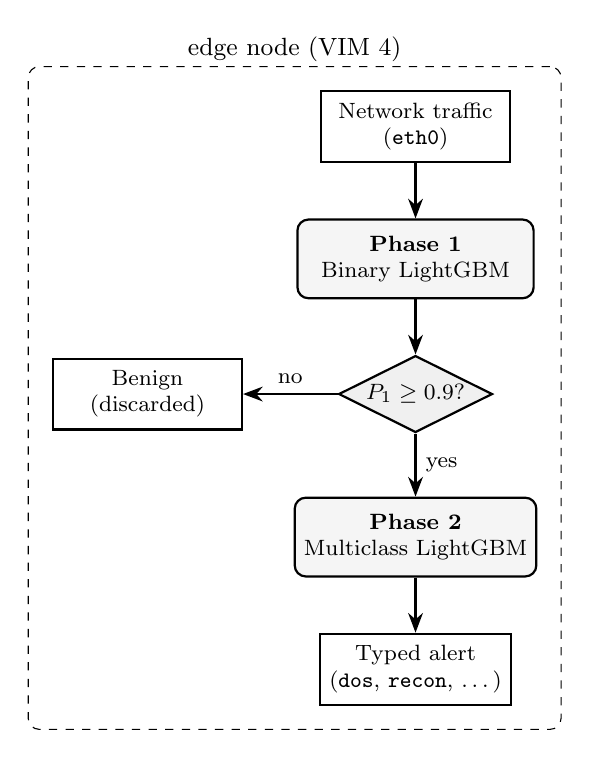
\begin{tikzpicture}[
  font=\footnotesize,
  box/.style={rectangle, rounded corners, draw, thick, align=center,
              minimum height=1.0cm, minimum width=3.0cm, fill=gray!8},
  dec/.style={diamond, aspect=2, draw, thick, align=center, fill=gray!12,
              inner sep=1pt},
  term/.style={rectangle, draw, thick, align=center, minimum height=0.9cm,
               minimum width=2.4cm},
  arr/.style={-{Stealth[length=2.5mm]}, thick}]
  \node[term] (traf) {Network traffic\\(\texttt{eth0})};
  \node[box, below=0.7cm of traf] (f1) {\textbf{Phase~1}\\Binary LightGBM};
  \node[dec, below=0.7cm of f1] (dec) {$P_1 \geq 0.9$?};
  \node[term, left=1.2cm of dec] (ben) {Benign\\(discarded)};
  \node[box, below=0.8cm of dec] (f2) {\textbf{Phase~2}\\Multiclass LightGBM};
  \node[term, below=0.7cm of f2] (tipo) {Typed alert\\(\texttt{dos}, \texttt{recon}, \ldots)};
  \draw[arr] (traf) -- (f1);
  \draw[arr] (f1) -- (dec);
  \draw[arr] (dec) -- node[above]{no} (ben);
  \draw[arr] (dec) -- node[right]{yes} (f2);
  \draw[arr] (f2) -- (tipo);
  \begin{scope}[on background layer]
    \node[draw, dashed, rounded corners, fit=(traf)(f1)(dec)(f2)(tipo)(ben),
          inner sep=0.30cm, label={[anchor=south, font=\small, yshift=-2pt]north:edge node (VIM~4)}] {};
  \end{scope}
\end{tikzpicture}}
\caption{Two-phase detection architecture.}
\label{fig:architecture}
\end{subfigure}
\hfill
\begin{subfigure}[b]{0.36\columnwidth}
\centering
\resizebox{!}{5.2cm}{%
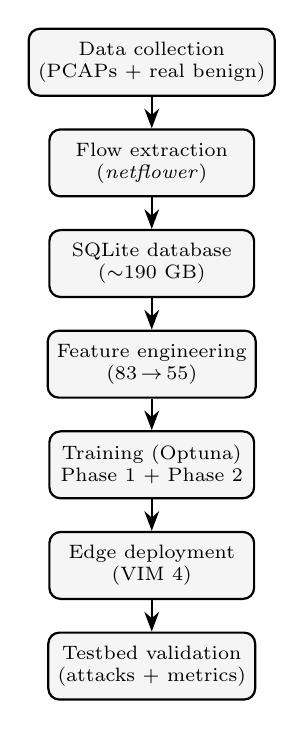
\begin{tikzpicture}[
  font=\scriptsize,
  stage/.style={rectangle, rounded corners, draw, thick, align=center,
                minimum height=0.85cm, minimum width=2.6cm, fill=gray!8},
  arr/.style={-{Stealth[length=2.5mm]}, thick}]
  \node[stage] (coleta)  {Data collection\\(PCAPs + real benign)};
  \node[stage, below=0.4cm of coleta] (flow)  {Flow extraction\\(\textit{netflower})};
  \node[stage, below=0.4cm of flow]   (db)    {SQLite database\\($\sim$190~GB)};
  \node[stage, below=0.4cm of db]     (feat)  {Feature engineering\\(83\,$\rightarrow$\,55)};
  \node[stage, below=0.4cm of feat]   (train) {Training (Optuna)\\Phase~1 + Phase~2};
  \node[stage, below=0.4cm of train]  (deploy){Edge deployment\\(VIM~4)};
  \node[stage, below=0.4cm of deploy] (val)   {Testbed validation\\(attacks + metrics)};
  \draw[arr] (coleta) -- (flow);
  \draw[arr] (flow)   -- (db);
  \draw[arr] (db)     -- (feat);
  \draw[arr] (feat)   -- (train);
  \draw[arr] (train)  -- (deploy);
  \draw[arr] (deploy) -- (val);
\end{tikzpicture}}
\caption{Methodology pipeline.}
\label{fig:methodology}
\end{subfigure}
\caption{Overview of the proposed system: (a) detection architecture and (b) end-to-end methodology, both on the edge node (VIM~4).}
\label{fig:overview}
\end{figure}

\subsection{Data pipeline}
\label{subsec:pipeline}

The database was built from datasets whose PCAPs are separated by category, with labels derived from folder names, which avoids schema
inconsistencies across sources~\cite{sharafaldin:18}. Two CIC datasets were
employed: the CIC IoT Dataset 2023~\cite{neto:23}, focused on multi-attack
traffic on IoT devices, and the CIC IIoT Dataset
2025\footnote{\url{https://www.unb.ca/cic/datasets/iiot-dataset-2025.html}}, which comprises industrial IoT intrusions. The benign class was complemented with real traffic captured by the authors over dozens of hours of everyday personal computer use (browsing, streaming, gaming, SSH sessions and system updates), converted into flows and labeled \texttt{benign}. The benign traffic of the CIC datasets is scripted, with regular temporal patterns, whereas real interactive traffic exhibits SSH bursts, HTTP keepalives and short flows over a fast local network. Mixing real traffic into training reduces the distribution shift between training and deployment.

Given the data scale (raw captures on the order of terabytes), each dataset is
consolidated into a single SQLite table, which is lightweight, portable and capable of performing aggregations and statistical queries directly on disk. The construction process is automated and reproducible: all PCAP files within each attack-category directory are converted into network flows by \textit{netflower} with eight parallel processes, and the resulting per-class CSV files are bulk-loaded into the database and indexed by the label column. By aggregating multiple packets into a single flow, a reduction
in the storage footprint by approximately 5× is achieved: the resulting database occupies $\sim$190~GB, compared with $\sim$1~TB  for the original PCAP files.


The \textit{netflower} is a flow-extraction tool developed in this work, published
on the Python Package Index
(PyPI)\footnote{\url{https://pypi.org/project/netflower/}} under the MIT
license~\cite{netflower}. From PCAPs or a live network interface, it
reconstructs bidirectional IPv4 flows (TCP/UDP) and produces 82
CICFlowMeter-compatible features (flow identity, duration and rate statistics,
packet-size and inter-arrival-time distributions, TCP-flag counts, active/idle
periods, bulk, subflow and initial-window metrics). Designed for edge devices,
it uses the \textit{dpkt} library (10--25$\times$ faster than Scapy on ARM),
accumulates statistics with Welford's online algorithm~\cite{welford} in
$O(1)$ memory per flow, accesses libpcap via \texttt{ctypes}, and emits each
flow only upon completion, by connection termination (TCP FIN/RST), inactivity
timeout (\texttt{idle\_timeout}, default 30~s) or maximum duration
(\texttt{flow\_timeout}, default 120~s). These two timeouts govern the
detection latency in live capture.

\subsection{Label mapping}
\label{subsec:labels}

Since DDoS and DoS attacks aim to exhaust resources and their network flows (high packet rate, short duration, flag anomalies) are similar, maintaining two separate classes may introduce noise without providing a significant discriminative gain for the classifier. Furthermore, from the perspective of the target node, the distinction between DoS and DDoS is not observable at the individual flow level. The received flows are statistically similar, while the main discriminative characteristic (source-IP diversity) requires aggregation across flows, which is not captured by the 55 per-flow features considered in this work. Therefore, we combined $\texttt{ddos}$ and  $\texttt{dos}$ attacks into a single class before training, reducing the space to 8 classes: \texttt{benign},
\texttt{dos} (resource exhaustion), \texttt{malware} (including Command and
Control communication), \texttt{bruteforce} (SSH, HTTP, Telnet), \texttt{mitm}
(ARP poisoning), \texttt{web} (application scanning and fuzzing),
\texttt{spoofing} (source forgery) and \texttt{recon} (network scanning).

\subsection{Feature engineering}
\label{subsec:features}

Starting from the 82 raw features generated by \textit{NetFlower}, a preprocessing stage removed the attribute groups that could cause the model to learn dataset-specific artifacts rather than intrinsic traffic characteristics: the features identifying specific hosts and services (e.g., IP addresses and port numbers), which lead the model to memorize endpoints observed during training instead of generalizable traffic patterns; the initial TCP window features carrying the sentinel value $-1$, which does not occur in real network traffic and could become a source of false positives; and the bulk-rate features, which \textit{NetFlower} always outputs as zero during live operation whereas the training datasets contain non-zero values, a discrepancy that would not exist in production. Two statistical filters completed this stage, discarding eleven highly correlated features ($|\rho| > 0.95$, Pearson) and three features with near-zero variance ($\sigma^2 < 10^{-4}$), which resulted in a final set of 55 numerical features. According to the LightGBM feature importance based on gain, the two most informative features were the flow byte rate per second (\texttt{flow\_byts\_s}) and the minimum packet inter-arrival time (\texttt{flow\_iat\_min}).


\subsection{Training the two phases}
\label{subsec:training}

The models comprising the two phases were trained independently using the SQLite database as the data source. The hyperparameters were optimized with Optuna, while class-balanced samples were extracted directly from the disk, avoiding the need to load the entire dataset into memory.

\subsubsection{Phase 1 - Binary classifier} The binary classifier was trained using 615,317 benign flows and all 554,795 attack flows. After duplicate removal, the resulting dataset comprised 703,558 unique instances, which were partitioned into training and test sets using a stratified 80/20 split. Hyperparameters and the decision threshold were jointly optimized with Optuna by maximizing the $F_2$-score, which assigns four times greater importance to recall than to precision, reflecting the significantly higher security cost of false negatives compared with false positives. Evaluation on the test set (140,712 flows) using the optimal decision threshold of 0.157 yielded an accuracy of 80\%, an attack recall of 96\%, a precision of 68\%, and an $F_2$ score of 88.6\%. Although this threshold provides interesting accuracy, recall, and  $F_2$ score, the resulting false-positive ratio, approximately one false alarm for every three alerts, is impractical for deployment in production environments. Therefore, the decision threshold was increased to 0.9 for operational use, sacrificing a small amount of recall to substantially reduce false positives (see Section~\ref{sec:results}).

\subsubsection{Phase 2 - Multiclass classifier}
The multiclass classifier was trained using independently sampled data, with the number of flows per attack category capped at 615,317. We applied  \texttt{class\_weight=balanced} to compensate for the scarcity of the \texttt{bruteforce} attack ($\sim$16k samples), while Optuna targeted the macro $F_1$ metric to weigh all classes equally. Table~\ref{tab:phase2_offline} summarizes the classifier performance considering the test set (317,381 flows), illustrating an offline baseline pattern that later intensifies on the physical testbed.
Specifically, \texttt{dos} traffic achieves near perfect classification ($F_1 = 98\%$), whereas \texttt{bruteforce}, \texttt{spoofing}, and \texttt{mitm} display low precision (20\%, 28\%, and 42\%) paired with high recall (72--77\%) driven by class balancing. A macro $F_1$ score of 67\% confirms that features extracted from an individual flow isolate attacks with distinct structural signatures effectively but perform poorly against volumetric floods.


%The multiclass classifier was trained using independently sampled data, with the number of flows per attack category capped at 615,317 to limit class imbalance. Additionally, the \texttt{class_weight=balanced} option was adopted to compensate for the scarcity of the \texttt{bruteforce} class (approximately 16,000 samples). Hyperparameters were optimized with Optuna by maximizing the macro-F


% score, thereby assigning equal importance to all attack categories regardless of their frequency. Table~\ref{tab:phase2_offline} reports the performance on the test set (317,381 flows), establishing the offline baseline that is subsequently compared with the results obtained on the physical testbed.




\begin{table}[t]
\centering
\caption{Phase~2 offline evaluation per class — test set.}
\label{tab:phase2_offline}
\footnotesize
\begin{tabular}{@{}lrrrr@{}}
\toprule
\textbf{Class} & \textbf{Precision} & \textbf{Recall} & \textbf{F1} & \textbf{Support} \\ \midrule
benign      & 83\% & 69\% & 76\% & 83{,}313 \\
bruteforce  & 20\% & 77\% & 31\% &  2{,}191 \\
dos         & \textbf{99\%} & \textbf{96\%} & \textbf{98\%} & 64{,}582 \\
malware     & 90\% & 78\% & 84\% & 81{,}338 \\
mitm        & 42\% & 72\% & 53\% & 13{,}823 \\
recon       & 83\% & 68\% & 75\% & 47{,}915 \\
spoofing    & 28\% & 73\% & 41\% & 12{,}289 \\
web         & 77\% & 84\% & 80\% & 11{,}930 \\ \midrule
\textbf{Accuracy} & & & \textbf{78\%} & 317{,}381 \\
Macro F1    & & & \textbf{67\%} & \\
\bottomrule
\end{tabular}
\end{table}

\subsection{Testbed validation: environment and protocol}
\label{subsec:validation}

The experimental validation was conducted using two machines connected to the same Gigabit Ethernet local network, shared with other hosts: a personal computer - PC (AMD Ryzen~5 7600, 32~GB DDR5 RAM, and an NVIDIA RTX~5070 GPU) and a Khadas VIM~4 board. The former was responsible for training the machine learning models (LightGBM on CPU), orchestrating the experiments via SSH, and generating attack traffic targeting the Khadas VIM~4. The latter served as the MEC node, executing the IDS on its \texttt{eth0} network interface. The Khadas VIM~4 is a low-cost edge computing platform suitable for IoT/MEC deployments, equipped with an Amlogic A311D2 system-on-chip (SoC) featuring eight heterogeneous ARM cores (4× Cortex-A73 at 2.2~GHz and 4× Cortex-A53 at 1.8~GHz), 8~GB of LPDDR4x RAM, and a 2.5--9~W power envelope.

%The validation involved two machines in an isolated Gigabit Ethernet local network: a personal computer (AMD Ryzen~5 7600, 32~GB DDR5, NVIDIA RTX~5070) and the Khadas VIM~4 board. The former was used to train the models (LightGBM on CPU), orchestrate the experiment over SSH, and generate  attacks targeting the Khadas VIM~4 board. The latter represents a MEC node and run the IDS at \texttt{eth0} interface. The VIM~4 gathers, in a low-cost single-board computer, the attributes of an access MEC node for IoT scenarios: an Amlogic A311D2 SoC with eight heterogeneous ARM cores (4$\times$ Cortex-A73 at 2.2~GHz and 4$\times$ Cortex-A53 at 1.8~GHz), 8~GB of LPDDR4x RAM and a 2.5--9~W power envelope.

On the PC, the orchestrator (\texttt{run\_experiment.sh}) deploys the scripts to the VIM~4 via SSH, coordinates the evaluation sessions and triggers the computation of the performance metrics. The attack generator (\texttt{attack\_generator.py}) sequentially executes the eight attack categories and produces a JSON report containing the time intervals associated with each attack, which serves as the ground-truth reference. The metrics script then correlates this report with the IDS logs collected from the VIM~4 to compute the detection metrics. 
On the VIM~4, the IDS (\texttt{network\_ids.py}) executes Phase~1 and, when enabled, Phase~2, logging per-flow detection events together with periodic snapshots of CPU utilization, memory usage, processor temperature, and operating frequency, from which the computational cost metrics are derived. The attacks use real tools, including 
nmap and masscan (SYN, UDP and aggressive scans), hping3 (SYN/UDP/ICMP floods, DDoS with random sources and spoofing with a forged source), medusa (SSH/HTTP/Telnet brute force), nikto and gobuster (web scanning and enumeration), curl (HTTP flood), arpspoof (bidirectional ARP poisoning for
MITM), and netcat (simulated C2 beacon). Brute force runs medusa over several
usernames and a generated password list, and the MITM step drives TCP and UDP
traffic through the poisoned route so that \textit{netflower}, which parses only
TCP and UDP, records it as flows.

The proposed approach is evaluated through two sequential sessions executed under the same script: Session~A enables only the binary IDS (Phase~1), whereas Session~B activates both classifiers (Phases~1 and~2), which isolates the incremental resource cost of the second phase. Each session begins and ends with a 60~s benign baseline period and includes a 120~s idle interval between consecutive attacks, which keeps the attack windows apart (labelling by flow start does not depend on this gap).
The binary classifier adopts a decision threshold of $P_1 \geq 0.9$. Detection is scored \emph{per flow}: each classified flow is labelled attack or benign according to the ground-truth window in which it \emph{started} (\texttt{flow\_ts}, the capture time of its first packet), never by when the alert was emitted. This is deliberate: under flooding the ARM node saturates and emits flows with a median delay of 181--428~s (Section~\ref{subsec:res_artifacts}), so any emission-anchored metric contaminates neighbouring seconds and windows. Two window definitions are reported: \emph{strict}, using the orchestrator's recorded start/end times, and \emph{calibrated} ($+2$~s), which widens each window by 2~s per side to correct a systematic lag. The orchestrator records \texttt{start\_time} after the attack tool is already sending, so the first attack flows begin up to $\sim$2~s before the logged instant, and 88\% of the strict false positives are exactly such real attack flows that the $+2$~s slack reabsorbs (the correction saturates at 2~s). Labelling remains by \texttt{flow\_ts}, without reintroducing emission time. For the multiclass classifier, the predicted category is the Phase~2 label when Phase~1 alerts, and benign otherwise. In addition to detection metrics, CPU utilization, RAM usage, alert throughput, and estimated energy consumption are reported for all experiments.

%─────────────────────────────────────────────────────────────────────────────
\section{Results}
\label{sec:results}

This section presents the experimental evaluation of the proposed hierarchical IDS deployed on the Khadas VIM4 platform under online attack traffic. The binary and multiclass configurations are systematically analyzed in terms of detection performance and computational, memory, and energy costs, guiding their deploying on resource-constrained edge nodes.

\subsection{Binary IDS (Phase 1)}
\label{subsec:res_bin}

Table~\ref{tab:bin_metrics} summarizes the binary-IDS results under the per-flow metric, over both strict and calibrated ($+2$~s) ground-truth windows. Under the calibrated window the detector reaches a precision of 96.8\%, a recall of 70.1\% and an F1 of 81.3\%. Under the strict window, these become 94.5\%, 69.6\% and 80.2\%. Precision is the reliable specificity measure in this testbed: as the capture is dominated by flooding ($\sim$99\% of flows are attack), genuinely benign traffic amounts to only a few hundred flows, so the FPR (42.3\% calibrated, 55.3\% strict) inherits a tiny, noisy denominator and is not comparable to an FPR measured on a clean benign baseline. The recall of 70\% reflects the operating threshold rather than a weak model: the single-packet UDP flows produced by the UDP floods score around 0.807, just below the 0.9 threshold, and count as misses.

\begin{table}[t]
\centering
\caption{Per-flow binary IDS metrics on the testbed (threshold 0.9), under strict
and calibrated ($+2$~s) ground-truth windows. Precision is the reliable
specificity measure. The FPR denominator is tiny (few hundred benign flows in a
flood-saturated capture).}
\label{tab:bin_metrics}
\footnotesize
\begin{tabular}{@{}lrr@{}}
\toprule
\textbf{Metric} & \textbf{Strict} & \textbf{Calibrated ($+2$~s)} \\ \midrule
Accuracy        & 67.9\% & \textbf{69.4\%} \\
Precision       & 94.5\% & \textbf{96.8\%} \\
Recall / TPR    & 69.6\% & \textbf{70.1\%} \\
F1-score        & 80.2\% & \textbf{81.3\%} \\
FPR             & 55.3\% & 42.3\% \\
FNR             & 36.0\% & 35.7\% \\
\bottomrule
\end{tabular}
\end{table}

Table~\ref{tab:detection_rate} shows that recall is unevenly distributed across attack types. Volumetric floods carrying a mix of TCP and UDP are detected well (spoofing 95.2\% and DoS 89.6\% of flows), but DDoS drops to 56.2\% because its random-source flood is dominated by single-packet UDP flows that score just below the threshold, and reconnaissance reaches 59.4\% because nmap's UDP scan emits too few packets per port to accumulate features before the flow expires (30~s \texttt{idle\_timeout}). Low-volume attacks are largely missed at this threshold: brute force 16.7\%, MITM 7.8\%, web 0.6\% and malware 2.9\%. These categories generate few flows by nature (brute force 233, MITM 193, malware 103), so their rates rest on small samples rather than on a generator artifact.

\begin{table}[t]
\centering
\caption{Per-flow recall per attack type, binary IDS, calibrated ($+2$~s) window (Section~\ref{subsec:res_bin}).}
\label{tab:detection_rate}
\footnotesize
\begin{tabular}{@{}lrrr@{}}
\toprule
\textbf{Attack} & \textbf{Flows} & \textbf{Detected} & \textbf{Recall} \\ \midrule
spoofing          & 148{,}763 & 141{,}664 & \textbf{95.2\%} \\
dos               & 166{,}428 & 149{,}028 & 89.6\% \\
ddos              & 456{,}514 & 256{,}523 & 56.2\% \\
recon             &   3{,}526 &   2{,}094 & 59.4\% \\
bruteforce        &      233 &      39 & 16.7\% \\
mitm              &      193 &      15 & 7.8\% \\
malware           &      103 &       3 & 2.9\% \\
web               &   8{,}168 &      51 & 0.6\% \\ \bottomrule
\end{tabular}
\end{table}

\subsection{Multiclass IDS (Phases 1+2)}
\label{subsec:res_multi}

All eight categories now generate flows (Table~\ref{tab:multi_metrics}). Phase~2 classifies \texttt{recon} well (F1 = 74.6\%), whereas the other attacks collapse onto \texttt{dos}, which absorbs most attack flows (precision 74.3\%, recall 51.2\%, F1 60.6\%). The 142{,}195 spoofing flows are labelled \texttt{dos} almost in full, and web, brute force, MITM and malware are essentially never assigned their own class. Type accuracy is 41.7\% (40.6\% strict) and macro-F1 over the attack classes is 19.4\%. Restricted to the flows Phase~1 detected, type accuracy rises to 64.3\%.

The type label thus identifies reconnaissance scans but does not separate the other attacks from generic flooding. Within the 55 per-flow attributes, short, high-rate flows are statistically indistinguishable from a flood. For \texttt{spoofing} the \texttt{dos} label is in fact appropriate, since the attack is a forged-source flood. Separating the rest would require state aggregated across flows, such as authentication-failure counts or source-IP diversity, which per-flow features lack by construction.

\begin{table}[t]
\centering
\caption{Multiclass IDS in the testbed (calibrated $+2$~s window; dos includes ddos).}
\label{tab:multi_metrics}
\footnotesize
\setlength{\tabcolsep}{3.5pt}
\begin{tabular}{@{}lrrrr@{}}
\toprule
\textbf{Class} & \textbf{Sup.} & \textbf{Prec.} & \textbf{Rec.} & \textbf{F1} \\ \midrule
recon      &   1{,}638 & 94.9\% & 61.4\% & \textbf{74.6\%} \\
dos        & 629{,}291 & 74.3\% & 51.2\% & 60.6\% \\
spoofing   & 142{,}195 &  6.9\% &  0.0\% & 0.0\% \\
web        &   8{,}131 & 100.0\% &  0.1\% & 0.2\% \\
bruteforce &      264 &  0.2\% &  0.4\% & 0.3\% \\
mitm       &      116 &  0.0\% &  0.9\% & 0.0\% \\
malware    &      103 &  0.0\% &  1.0\% & 0.0\% \\ \midrule
\textbf{Type accuracy} & \multicolumn{4}{r}{\textbf{41.7\%} (40.6\% strict)} \\
\textbf{Macro F1 (attacks)} & \multicolumn{4}{r}{19.4\%} \\
\bottomrule
\end{tabular}
\end{table}



\subsection{Distribution shift and deployment artifacts}
\label{subsec:res_artifacts}

Three deployment phenomena, absent from offline evaluation, help explain the results. The most consequential is a throughput ceiling. At about 1{,}050 flows/s the ARM node cannot process traffic in real time: the inference queue grows to a peak of 433{,}469 flows for the binary pipeline and 491{,}880 for the hierarchical one, RAM rises to 2.4--2.6~GB, and the mean end-to-end latency from capture to classification is 116~s and 343~s respectively, with maxima of 182~s and 550~s. Because the queue is unbounded and fully drained at shutdown, no captured flow is dropped, so the overload surfaces as latency and memory rather than packet loss. Scoring by flow start (\texttt{flow\_ts}) makes the detection metrics immune to this displacement, which changes \emph{when} an alert appears, not \emph{which} flow it is. The second phenomenon is a distribution shift in benign traffic: \texttt{flow\_iat\_min} lies in the millisecond range in training but drops to 1--10~µs in real TCP bursts, which argues for capturing benign traffic in the deployment environment itself. The third is a \textit{netflower} artifact: each TCP teardown produces a single-packet FIN/ACK micro-flow scored at $\sim$84\% attack probability, mitigated by a minimum-packet guard before inference.


\subsection{Binary IDS vs.\ multiclass IDS}
\label{subsec:res_comp}

Table~\ref{tab:comparison} compares both configurations. The two columns are the two independent testbed sessions, which share the Phase~1 model but generate their own attack traffic. Each session drains its queue completely before exiting, so the flow totals (827{,}458 vs 809{,}448) carry no dropped residual; the $\sim$2\% gap is almost all benign background, as the attack traffic is nearly identical (783{,}928 vs 781{,}738, 0.3\%). Adding Phase~2 is far from free on this node. Average CPU rises from 12.3\% to 41.6\% (peaks 43\% to 73\%), average power during attacks from 3.49 to 5.20~W, and the mean end-to-end latency from 116 to 343~s, while peak RAM grows by about 157~MB to 2.61~GB. Batched inference itself is cheap (0.14~ms per flow in Phase~1 and 1.22~ms in Phase~2), so the cost comes from Phase~2 running on the traffic Phase~1 flags, not from the model.


\begin{table}[t]
\centering
\caption{Pipeline comparison on the VIM~4 platform. Columns are the two
independent testbed sessions (they share the Phase~1 model but generate their own
attack traffic, so Phase~1 metrics differ). $^\dagger$The FPR denominator is tiny
(few hundred benign flows in a flood-saturated capture); precision is the reliable
specificity measure.}
\label{tab:comparison}
\setlength{\tabcolsep}{4pt}
\footnotesize
\begin{tabular}{@{}lrr@{}}
\toprule
\textbf{Metric} & \shortstack[r]{\textbf{Binary}\\ \textbf{(Phase~1)}}
                 & \shortstack[r]{\textbf{Multiclass}\\ \textbf{(Phases~1+2)}} \\ \midrule
\multicolumn{3}{l}{\textit{Binary detection (Phase 1), per flow, $+2$~s window}} \\
\quad Precision            & \textbf{96.8\%} & 97.4\% \\
\quad Recall / TPR         & \textbf{70.1\%} & 64.3\% \\
\quad F1-score             & \textbf{81.3\%} & 77.5\% \\
\quad Accuracy             & \textbf{69.4\%} & 63.9\% \\
\quad FPR\rlap{$^\dagger$} & 42.3\%         & 47.8\% \\ \midrule
\multicolumn{3}{l}{\textit{Type classification (Phase 2)}} \\
\quad Accuracy (type)   & —               & \textbf{41.7\%} \\
\quad Macro F1 (attacks) & —            & 19.4\% \\ \midrule
\multicolumn{3}{l}{\textit{Resources (VIM 4, during session)}} \\
\quad CPU avg / max     & 12.3\% / 43.0\% & \textbf{41.6\% / 72.8\%} \\
\quad RAM avg           & 1{,}866 MB      & 2{,}041 MB \\
\quad RAM max           & 2{,}449 MB      & 2{,}606 MB (\textbf{+157 MB}) \\ \midrule
\multicolumn{3}{l}{\textit{Throughput and latency}} \\
\quad Flows classified  & 827{,}458 & 809{,}448 \\
\quad Alerts emitted    & 567{,}836 & 516{,}182 \\
\quad Attack traffic    & $\sim$985 flows/s & $\sim$1{,}050 flows/s \\
\quad Queue peak        & 433{,}469 & 491{,}880 \\
\quad Mean e2e latency  & 116~s & \textbf{343~s} \\ \midrule
\multicolumn{3}{l}{\textit{Estimated energy}} \\
\quad Avg.\ power (attack) & 3.49~W & \textbf{5.20~W} \\
\quad Avg.\ power (idle)   & 2.77~W & 4.81~W \\
\quad Total energy (band)  & 4{,}375--6{,}672~J & 6{,}478--10{,}043~J \\
\bottomrule
\end{tabular}
\end{table}


The energy consumption in Table~\ref{tab:comparison} is a calibrated estimate,
not a direct measurement, since the VIM~4 exposes no energy telemetry
interfaces (RAPL or an INA226 sensor). Power is modeled linearly on CPU
utilization,
\begin{equation}
P(t) = P_{idle} + (P_{max} - P_{idle}) \times \text{CPU\%}(t),
\label{eq:power}
\end{equation}
with $P_{idle} = 2.5$~W and $P_{max} = 9.0$~W anchored on the VIM~4 power
envelope, calibrated at rest and under full load, and integrated over the
periodic samples ($\sim$3~s), separating attack from idle by the ground-truth
windows. The resulting sensitivity band is 4{,}375 to 6{,}672~J for the binary
pipeline and 6{,}478 to 10{,}043~J for the multiclass one. What matters is the
relative comparison: the hierarchical pipeline raises average power during
attacks from 3.49 to 5.20~W, a direct consequence of Phase~2's CPU load under
flooding rather than a memory-only overhead.

%─────────────────────────────────────────────────────────────────────────────
\section{Conclusion}
\label{sec:conclusion}

This work presented a two-phase hierarchical IDS for IoT environments in 6G
networks with MEC, from data pipeline to deployment and testbed validation on
the VIM~4 board. Scored per flow, the binary IDS detected volumetric floods
precisely (spoofing 95\%, DoS 90\%) at a precision of 97\%, while low-volume
attacks and single-packet floods fall below the 0.9 threshold and lower the
overall recall to 70\%. Phase~2 separates reconnaissance but merges the other
flood-like attacks into \texttt{dos}, a boundary of per-flow features rather
than a pipeline fault. The main operational finding is a throughput ceiling: at
$\sim$1{,}050 flows/s the VIM~4 cannot keep up and buffers traffic with a
latency of minutes, and adding Phase~2 roughly triples that latency while
raising CPU and power, so the hierarchical pipeline as deployed does not sustain
line-rate detection under volumetric attack on this node. Future work includes
bounding the queue with load shedding or sampling under overload, parallelizing
inference across the node's cores, adding aggregate cross-flow features to
separate flood-like attacks, evaluating against real services to reduce the
training-to-production shift, and replacing the energy estimate with hardware
measurements. The scripts and trained models are available in an open
repository\footnote{\url{https://github.com/luiz-linkezio/A-Hierarchical-Solution-based-on-MEC-and-IoT-for-Cyberattack-Detection-in-6G-Networks}}.

%─────────────────────────────────────────────────────────────────────────────
\bibliographystyle{IEEEtran}
\bibliography{artigo}

\end{document}
